\chapter{Les gerbes hadroniques et électromagnétiques}
\label{chap.shower}
Lorsqu'une particule traverse de la matière, elle va généralement interagir avec celle-ci. Cet interaction peut prendre différentes formes mais sera accompagné d'une perte d'énergie de la particule incidente. À très haute énergie, dans les milieux dense, les phénomènes de gerbes électromagnétiques ou hadroniques s'observent selon la nature de la particule incidente. Le but de ce chapitre est de décrire ces deux phénomènes. Dans un premier temps, nous détaillerons les différents types d'interaction rencontrer dans les gerbes hadroniques et électromagnétiques. Ceci nous permettra d'expliquer ces phénomènes et d'expliquer leurs propriétés importantes.
\minitoc
\newpage

%%%%%%%%%%%%%%%%%%%%%%%%%%%%%%%%%%%%%%%%%%%%%%%

\section{Interaction des particules avec la matière}
\label{sec.particle_in_matter}
\subsection{Interactions des particules chargées}
\label{sec.charged_in_matter}
Les particules chargées interagissent avec la matière de plusieurs façons. Les particules peuvent ioniser les atomes du milieu si leur énergie est suffisante pour leur arracher un électron. Après, le passage d'une particule chargée, les atomes peuvent être dans un état excité. Ces atomes se désexcitent en émettant un rayonnement appelée scintillation. Ces deux types d'interaction sont largement utilisés pour la conception de détecteurs. Les détecteurs gazeux utilisent les électrons issus des ionisations qui après amplification permettent d'obtenir un signal visible. Les scintillateurs collectent les photons émis vers des photomultiplicateurs pour détecter les particules. La valeur moyenne de la perte d'énergie $\big<dE/dx\big>$ par unité de longueur des particules chargées est donnée par la formule de Bethe-Block:
\begin{equation}
  \big<-\frac{dE}{dx}\big>=Kz^2\frac{Z}{A}\frac{1}{\beta^2}\big[\frac{1}{2}ln\frac{2m_ec^2\beta^2\gamma^2T_{max}}{I^2}-\beta^2-\frac{\delta(\beta\gamma)}{2}\big]
\label{eq.bethe}
\end{equation}
où $z$ est le nombre de charge du projectile, $Z$ le numéro atomique de la cible, $T_{max}$ est l'énergie cinétique maximale que peut emporter un électron après une collision, $I$ est le potentiel d'excitation moyen du matériau et $\delta$ est un facteur de correction pour prendre en compte la densité du matériau. La constante $K$ vaut $4\pi N_Ar_e^2m_ec^2$, $\gamma$ est la facteur de Lorentz $\frac{1}{\sqrt{1-\beta^2}}$ et $\beta$ vaut $\frac{v}{c}$.
\begin{figure}[!h]
  \begin{center}
    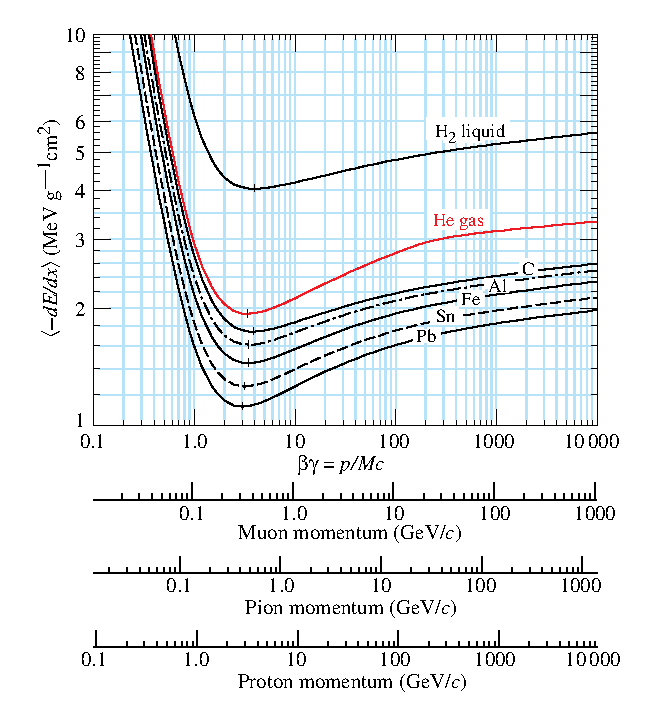
\includegraphics[width=.6\textwidth]{ShowerTh/figs/dedx_table_98.eps}
    \caption{Perte d'énergie de particules chargées dans de l'hydrogène liquide, de l'hélium gazeux, du carbone, de l'aluminium, du fer, de l'étain et du plomb en fonction de $\beta\gamma$. Le facteur $\beta\gamma$ est converti en énergie pour les muons, les pions et les protons. Les effets radiatifs ne sont pas inclus.}
    \label{fig:charged_in_matter}
  \end{center}
\end{figure}
Cette équation est valable dans la gamme $0.1\leq\beta\gamma\leq1000$ avec une erreur inférieur de 1$\%$. Cette formule nécessite quelques modifications pour décrire la perte d'énergie par unité de longueur pour les électrons et les positrons. Les électrons et les positrons subissent des diffusions dans le milieu. Les électrons déposent de l'énergie via la diffusion M{\o}ller ($e^-e^-\rightarrow e^-e^-$) et les positrons via la diffusion BhaBha ($e^+e^-\rightarrow e^+e^-$). Les positrons de basse énergie (E<100 $MeV$) peuvent aussi s'annihiler avec les électrons des atomes du milieu. Cette annihilation entraîne l'émission de deux photons d'énergie au moins supérieur à 511 $keV$.

La figure~\ref{fig:charged_in_matter} montre la perte d'énergie de particules chargées en fonction de $\beta\gamma$ pour plusieurs matériaux. Les effet radiatifs (Bremsstrahlung) ne sont pas pris en compte sur cette figure. Ces effets deviennent important pour des muons dans le fer à partir de 100 $GeV$ \cite{pdg}. En effet, lorsque l'énergie augmente, le rayonnement de freinage ou Bremsstrahlung doit être pris en compte. À haute énergie, les particules interagissent avec le champ électrique créé par les noyaux du milieu. Les particules sont déviées par ce champ, ce qui entraîne l'émision de photons. L'énergie perdu par unité de longueur en rayonnement de freinage est donnée par la formule:
\begin{equation}
  \frac{dE}{dx}~=~4\alpha N_A~\frac{z^2Z^2}{A}~\big(\frac{1}{4\pi\varepsilon_0}\frac{e^2}{mc^2}\big)^2~E~ln\frac{183}{Z^{\frac{1}{3}}}~\propto~\frac{E}{m^2}
\end{equation}
Cette énergie perdue est inversement proportionnelle au carré de la masse de la particule incidente. Le rapport $m_{\mu}^2/m_e^2\simeq40000$ indique que cet effet est négligeable pour des particules plus massives que l'électron jusqu'à une certaine énergie donnée. La masse de l'électron étant très faible, le rayonnement de freinage sera rapidement l'interaction dominante pour les électrons et les positrons lorsque l'énergie augmente. 
\begin{figure}[!h]
  \begin{center}
    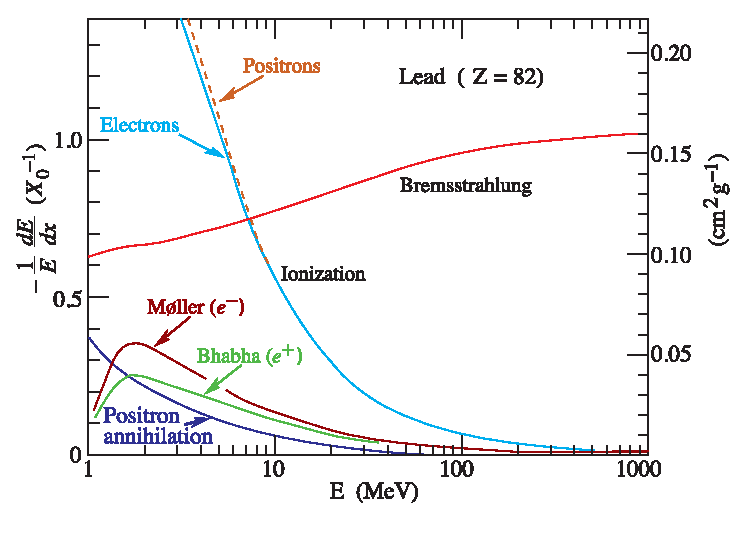
\includegraphics[width=.6\textwidth]{ShowerTh/figs/elossfrac_06.eps}
    \caption{Fraction d'énergie perdue par unité de longueur de radiation pour des électrons et des positrons dans du plomb. }
    \label{fig:electron_in_lead}
  \end{center}
\end{figure}
 La figure~\ref{fig:electron_in_lead} présente la fraction d'énergie perdue par unité de longueur de radiation $X_0$ (voir section~\ref{sec.x0}) pour des électrons et des positrons en fonction de leur énergie dans du plomb \cite{pdg}. Les différentes contributions à la perte d'énergie sont indiquées avec des couleur différentes. Le point correspondant à l'énergie où la perte d'énergie par Bremsstrahlung est plus importante que par ionisation est appelé énergie critique $\epsilon_c$. L'énergie critique varie comme $1/Z$, avec $Z$ le numéro atomique de l'élément.

\subsection{Interactions des photons}
\label{sec.photon_in_matter}
Les processus d'interaction des photons dans la matière sont les suivants: l'effet photoélectrique, l'absorption photo-nucléaire, la diffusion Rayleigh, la diffusion Compton et la création de paire. La section efficace de ces processus varie fortement avec l'énergie du photon incident. 
\subsubsection{Effet photoélectrique}
L'effet photoélectrique a été mis en évidence par Hertz en 1887. Il correspond à l'émission d'électrons par un matériau soumis à un rayonnement. Pour éjecter un électron de sa couche, il faut que l'énergie du photon soit supérieur à l'énergie de liaison de l'électron. Ce phénomène est le processus avec la plus grande section efficace pour des photons de basse énergie. La section efficace de l'effet photoélectrique varie comme $1/E$ mais présente des sauts lorsque l'énergie du photon incidents est égal à l'énergie de liaison d'une couche électronique.
\subsubsection{Diffusion Rayleigh}
La diffusion Rayleigh est un processus élastique: les photons ne perdent pas d'énergie. Cependant, la trajectoire des photons est modifiée à cause des couches électroniques des atomes. Ce processus a une section efficace relativement importante à basse énergie.
\subsubsection{Diffusion Compton}
Lors d'une diffusion Compton, le photon incident est dévié par la couche électronique d'un atome avec un transfert d'énergie du photon vers un électron. Cette énergie est suffisante pour que l'électron ne soit plus lié à l'atome. La figure~\ref{fig:compton_scattering} présente un schéma de diffusion Compton. Ce processus est l'interaction dominante pour des énergie intermédiaire (voir figure~\ref{fig:photon_in_matter}).
\begin{figure}[!h]
  \begin{center}
    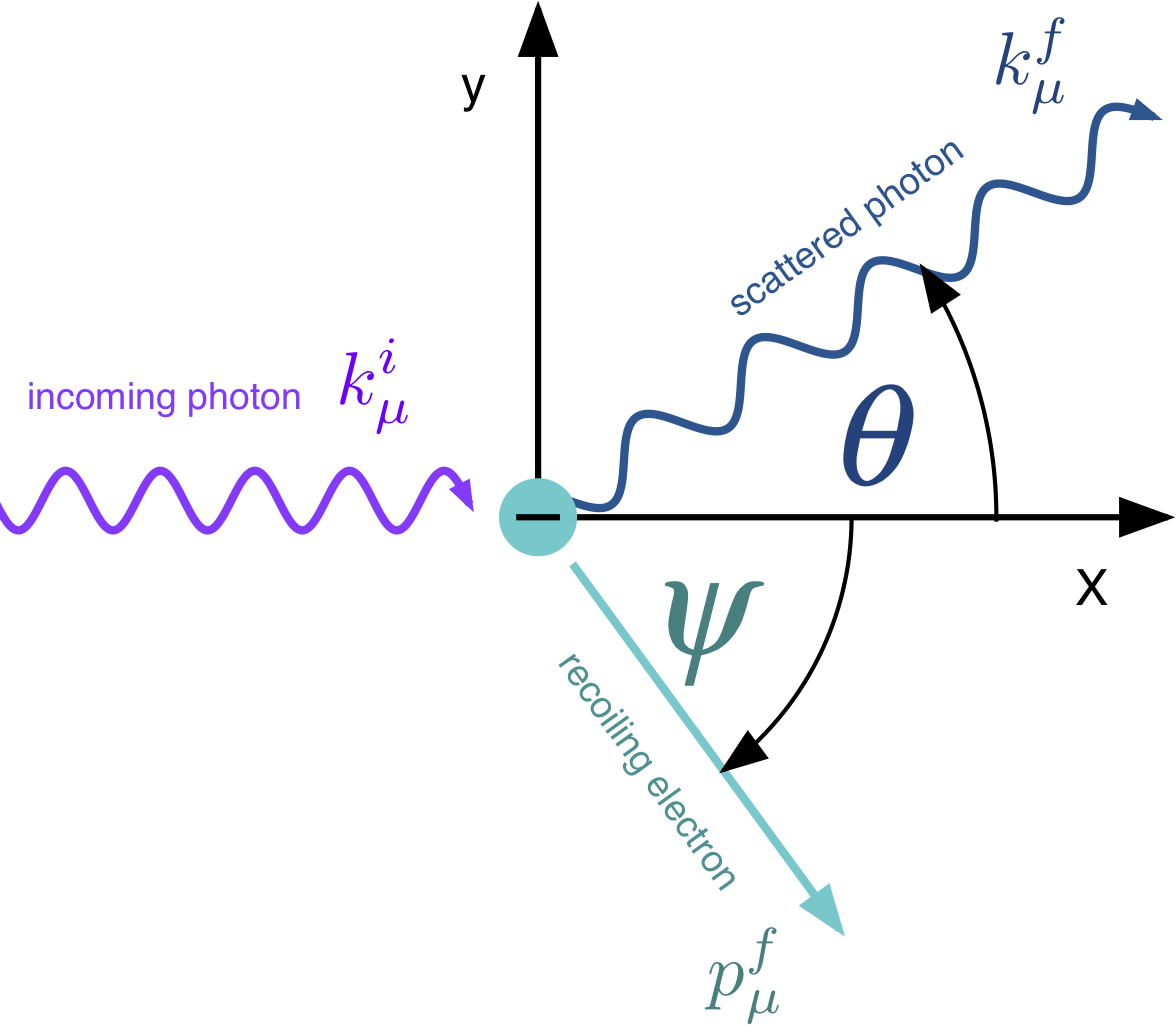
\includegraphics[width=.4\textwidth]{ShowerTh/figs/compton_scattering.png}
    \caption{Schéma explicatif de la diffusion Compton.}
    \label{fig:compton_scattering}
  \end{center}
\end{figure}
La variation de longueur d'onde du photon est donnée par l'équation suivante:
\begin{equation}
  \label{eq.compton}
  \lambda_i-\lambda_f=\frac{h}{m_ec}(1-cos\theta)
\end{equation}
où $\lambda_i$ est la longueur d'onde du photon incident, $\lambda_f$ la longueur d'onde du photon après la diffusion et $\theta$ l'angle de diffusion. En pratique, un photon dans un matériau va subir plusieurs diffusions Compton (si son énergie est suffisante) et donc perdre son énergie en plusieurs étapes. Lorsque son énergie sera suffisamment faible, le photon sera absorbé par un atome grâce à l'effet photoélectrique. 

\subsubsection{Ineraction photonucléaire}
Pour des énergies comprises entre 5 et 20 $MeV$, les photons peuvent interagir avec les nucléons des noyaux du milieu. Les photons sont absorbés par des neutrons, des protons ou induisent des fissions nucléaires \cite{wigmans}. La section efficace de ces processus est assez faible et ne dépasse pas 1$\%$ de la section efficace totale (voir figure\ref{fig:photon_in_matter}).

\subsubsection{Création de paire}
À plus haute énergie, le processus ayant la plus grande section efficace est le processus de création de paire. Lorsque l'énergie du photon est au moins supérieure à 2 fois la masse de l'électron, une paire électron-positron peut être créée. La plupart des conversion $\gamma\rightarrow e^+e^-$ sont dus aux champ électromagnétique d'un noyau. Pour des milieux de faible $Z$, le champ électromagnétique créé par les couches électroniques des atomes peut engendrer des création de paire. Si l'énergie du photon incident est suffisante, les électrons et les positrons rayonneront d'autre photons via le processus de Bremsstrahlung ou perdront leur énergie via les processus décrit précédemment.

La figure~\ref{fig:photon_in_matter} présente la section efficace totale en fonction de l'énergie des photons dans du carbone et du plomb. 
\begin{figure}[!h]
  \begin{center}
    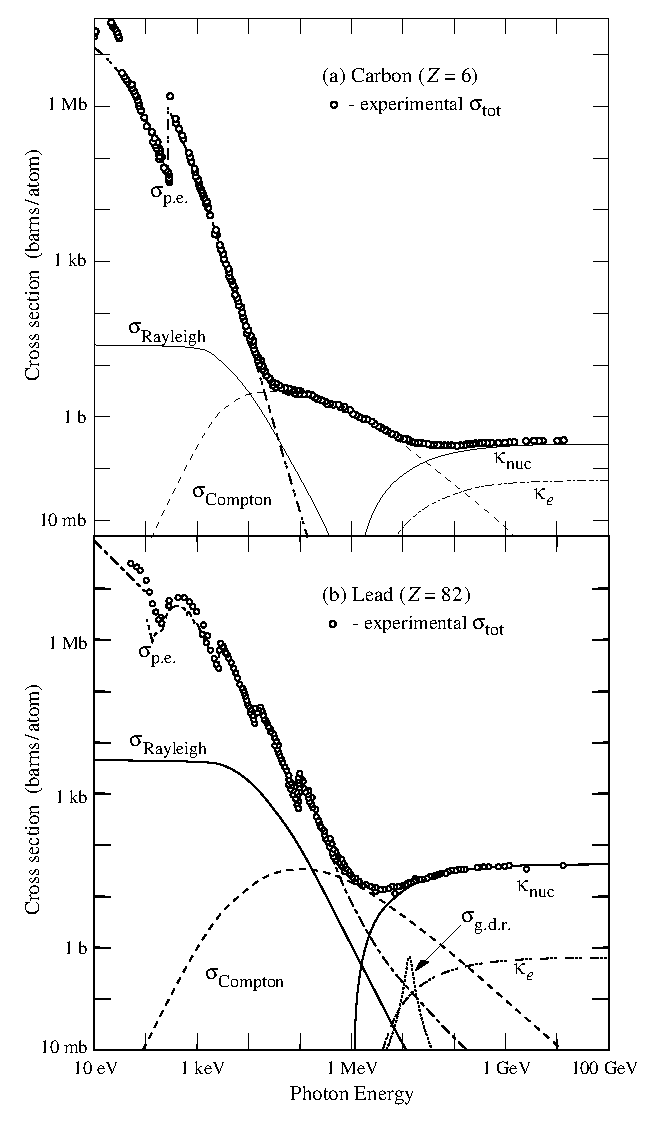
\includegraphics[width=.6\textwidth]{ShowerTh/figs/sigma_both_06.eps}
    \caption{Section efficace totale en fonction de l'énergie des photons dans du carbone (en haut) et du plomb (en bas).}
    \label{fig:photon_in_matter}
  \end{center}
\end{figure}
Les courbes théoriques de chacun des processus décrit dans les sous sections précédentes sont indiquées. Les données expérimentales sont représentées par des cercles. $\sigma_{p.e.}$ représente la section efficace de l'effet photoélectriques; $\sigma_{Rayleigh}$ et $\sigma_{Compton}$ les sections efficaces des diffusions Rayleigh et Compton; $\sigma_{g.d.r}$ la section efficace des processus photo-nucléaire; $\kappa_{nuc}$ et $\kappa_e$ les sections efficaces des créations de paires avec le champ électromagnétique du noyau et des électrons des atomes.

\subsection{Interaction des hadrons}
Les réactions possibles des hadrons avec la matières sont plus compliquées que pour les muons, les électrons et les photons car les hadrons sont soumis à l'interaction forte. Certains d'entre eux se désintègrent électromagnétiquement. C'est le cas des $\pi_0$ et $\eta$ qui se désintègrent majoritairement en photons. Les désintégrations de ces deux mésons ne sont pas dus à des interaction avec la matière mais à leur temps de vie très court ($t_{0,\pi_0}=8.4\times 10^{-17}\ s$ et $t_{0,\eta}=5.0\times 10^{-19}\ s$). Cependant, ils seront produits assez abondement dans les gerbes hadroniques et leurs produits de désintégration ineragissent avec la matière. 

Un hadrons chargé de haute énergie ($E>10\ GeV$) perd son énergie par ionisation (voir section~\ref{sec.charged_in_matter}) jusqu'à une certaine profondeur où il interagit fortement avec un noyau du milieu. Dans ces réactions avec les noyaux, les hadrons peuvent changer de nature et de nombreux nouveaux hadrons peuvent être émis. Les noyaux de la réaction peuvent aussi perdre de nombreux nucléons et émettre des $\gamma$s. Les hadrons neutres ne déposent pas d'énergie par ionisation. Pour ces particules, la perte d'énergie dans la matière se fait uniquement avec des interaction avec les noyau du milieu. 
\begin{figure}[!h]
  \begin{center}
    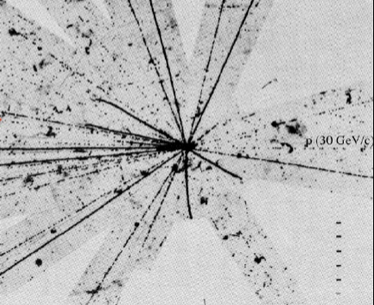
\includegraphics[width=.6\textwidth]{ShowerTh/figs/nuclear_reaction_emulsion.png}
    \caption{Photographie d'une réaction induite par un proton de 30 GeV avec un noyau dans une émulsion nucléaire.}
    \label{fig:hadron_nucleus_interaction}
  \end{center}
\end{figure}
La figure~\ref{fig:hadron_nucleus_interaction} montre une photographie d'une réaction entre un proton de 30 GeV et un noyau d'une émulsion nucléaire. Une vingtaine de particules chargées sont produites de façon plus ou moins isotrope. 

Le mécanisme de spallation nucléaire décrit l'interaction des hadrons d'énergie entre 50 $MeV$ jusqu'à quelques $GeV$, avec la matière . La spallation nucléaire est décrites en deux étapes \cite{wigmans}. La première consiste en une rapide cascade intranucléaire: une collision entre un hadron de haute énergie et un ou plusieurs nucléons d'un noyau s'opère; ces nucléons font de nouvelles collisions avec les autres nucléons du noyau. Des hadrons instables peuvent aussi être créer à ce stade si l'énergie est suffisante. Certaines particules de la cascade s'échappent du noyau. La deuxième étapes de la spallation nucléaire consiste à la désexcitation du noyau. Cette désexcitation prend généralement la forme d'évaporation d'un ou plusieurs nucléons. Des particules $\alpha$s peuvent aussi être évaporées. Le processus d'évaporation prend fin lorsque l'énergie est inférieur à l'énergie de liaison des nucléons. Si le noyau est toujours dans un états excités des $\gamma$s peuvent être émis. Dans le cas des noyaux très lourd, des fissions peuvent avoir lieu. 
\subsection{Interaction des neutrons}
Les interaction des neutrons avec la matière sont très différentes de celle avec les autres particules. En effet, les neutrons n'interagissent avec la matière uniquement via l'interaction forte et parfois faible. Étant neutre, ils ne déposent pas d'énergie par ionisation mais ils peuvent initiés des réactions de spallation lorsqu'ils ont suffisamment d'énergie. À basse énergie les neutrons peuvent être diffusés ou absorbés.
\subsubsection{Diffusion élastique des neutrons}
La diffusion élastique ou quasi-élastique des neutrons dans la matière est le processus majoritaire de perte d'énergie pour des neutrons d'énergie inférieure à 10 $MeV$. Les neutrons font des collisions avec des noyaux et transfèrent une partie de leur énergie cinétique. Les sections efficaces de ces collisions varient en fonction du matériau mais le libre parcours moyen de ces neutrons est généralement de quelques $cm$. La fraction d'énergie perdu lors de ces diffusions varie de 0 à $4A/(A+1)^2$, où $A$ est le numéro atomique. La fraction d'énergie perdue moyenne est de 50$\%$, 3.4$\%$,et 0.96$\%$ pour l'hydrogène, le fer et le plomb. Les calorimètres hadroniques dont la partie active est faite de scintillateurs en plastique sont très sensibles aux neutrons. Ceci est à la fois un avantage et un inconvénient. Les dépôts d'énergie dus au neutrons permettent d'améliorer la résolution en énergie de ces calorimètres. Cependant, ces neutrons peuvent voyager longtemps dans les absorbeurs et induire un signal avec du retard et/ou éloigné du dépôt principal, ce qui peut entraîner une confusion. 
\subsubsection{Diffusion inélastique des neutrons}
Pour des énergies situées entre 10 et 100 $MeV$, les neutrons déposent leur énergie avec des diffusions inélastiques. Contrairement aux diffusions élastiques, les noyaux cibles sont dans un états excités après l'interaction avec le neutron incident. Ces noyaux se désexcitent selon plusieurs processus en fonction de l'énergie transférée par le neutron incident. Le retour à l’état stable des noyaux prend la forme d'émissions de rayonnements $\gamma$s, de protons, de neutrons et de particules $\alpha$s. Une fission du noyau cible peut aussi être déclenchée. 
\subsubsection{Capture de neutrons}
Lorsqu'un neutron a perdu presque toute son énergie cinétique, il peut être capturé par un noyau. Le nouveau noyau est dans un état excité. Des émissions d'un $\gamma$ ou d'une particule $\alpha$ permettent de retrouver l'état stable.

\section{Gerbes électromagnétiques}

\subsection{Cascades électromagnétiques}
Prenons l'exemple d'une cascade initié par un électron pour décrire le phénomène de gerbe électromagnétique. Lorsqu'un électron de haute énergie traverse un matériau le rayonnement de freinage est de loin son mode privilégié de perte d'énergie (cf. figure~\ref{fig:charged_in_matter}). Ces photons vont se convertir en paires électron-positron qui vont à leur tour perdre de l'énergie sous forme de rayonnement. Ces interactions créent un phénomène de cascade. Les photons peuvent se convertir en paire tant que leur énergie est supérieur à 1022 $keV$. La cascade se terminera avec les processus de basse énergie comme la diffusion Compton, l'effet photoélectrique, l'annihilation de positron...
\begin{figure}[!h]
  \begin{center}
    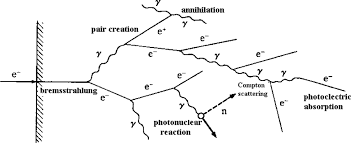
\includegraphics[width=.4\textwidth]{ShowerTh/figs/electromagnetic_cascade.png}
    \caption{Schéma d'une cascade électromagnétique initiée par un électron de haute énergie.}
    \label{fig:electromagnetic_cascade}
  \end{center}
\end{figure}
La figure~\ref{fig:electromagnetic_cascade} est un schéma d'une cascade électromagnétique initiée par un électron de haute énergie. Les cascades électromagnétiques peuvent aussi être initiées par des photons de haute énergie. Les pions neutre $\pi_0$ peuvent aussi être le point de départ d'une telle cascade. Le temps de vie des pions neutres est très faibles ($t_0=8.4\pm 0.5\times 10^{-17}s$) et ils se désintègrent à 99$\%$ en paire de photons qui déclencheront des cascades électromagnétiques. Nous verrons dans la section~\ref{sec.hadron_shower} que des pions neutres sont créés dans les gerbes hadroniques. Ceux-ci déclencheront des cascades électromagnétiques. On parlera alors de fraction électromagnétique dans les gerbes hadroniques.

\subsection{Longueur de radiation}
\label{sec.x0}
Une propriété importante des matériaux pour les gerbes électromagnétiques est la longueur de radiation $X_0$. Cette longueur correspond à la longueur moyenne pour qu'un électron de haute énergie (>>1$GeV$) dépose une fraction $1/e$ ($\simeq 63\%$) de son énergie. La longueur de radiation est souvent exprimée en $g.cm^2$. Il suffit de diviser par la densité du matériau pour obtenir une grandeur homogène à une longueur. L'équation suivante donne la longueur de radiation en fonction des paramètres du matériau \cite{pdg}: 
\begin{equation}
  \frac{1}{X_0}=4\alpha r_e^2\frac{N_A}{A}\big\{Z^2\big[L_{rad}-f(Z)\big]+ZL'_{rad}\big\}
  \label{eq.x0}
\end{equation}
où $\alpha$ est la constante de structure fine, $r_e$ le rayon classique de l'électron ($r_e=\frac{1}{4\pi\varepsilon_0}\frac{e^2}{m_ec^2}$), $N_A$ le nombre d'Avogadro, $A$ est la masse atomique (en $g.mol^1$), $Z$ le numéro atomique. $L_{rad}$ et $L'_{rad}$ et $f(z)$ dépendent du numéro atomique de l'élément. Le tableau~\ref{tab.x0} indique la longueur de radiation pour différents éléments \cite{pdg}.
\begin{table}[!ht]
  \begin{center}
    \begin{tabular}{c|c|c|c}
      Matériau & Densité ($g.cm^{-3}$) & $X_0$ ($g.cm^{-2}$) & $X_0$ (cm)\\
      \hline
      Eau & $1$ & $36.08$ & $36.08$ \\
      Carbone (graphite) & $2.265$ & $42.70$ & $18.8$\\
      Fer & $7.87$ & $13.84$ & $1.76$\\
      Plomb & $11.35$ & $6.37$ & $0.56$\\
      Tungsten & $19.3$ & $6.76$ & $0.35$
    \end{tabular}
  \end{center}  
  \caption{Longueur de radiation pour différents matériaux.}
  \label{tab.x0}
\end{table}

\subsection{Le rayon de Molière}
Le rayon de Molière $R_M$ est régulièrement utilisé pour décrire le développement transversale des gerbes électromagnétiques. Il est défini avec l'équation suivante \cite{pdg}:
\begin{equation}
  R_M=X_0\frac{E_s}{\epsilon_c}
\end{equation}
où $E_s=m_ec^2\sqrt{4\pi/\alpha}\simeq 21.2~MeV$, et $\epsilon_c$ l'énergie critique (voir section~\ref{sec.charged_in_matter}). En moyenne 90$\%$ de l'énergie déposée dans une gerbe hadronique se fait dans un cylindre de $R_M$ autour de l'axe de la gerbe \cite{wigmans}.

\subsection{Profiles des gerbes électromagnétiques}
Le profile longitudinal d'une gerbe électromagnétique correspond à la quantité d'énergie déposée en fonction de la profondeur de matériau traversé. La profondeur est souvent exprimée en fonction de la longueur de radiation $X_0$.
\begin{figure}[!h]
  \begin{center}
    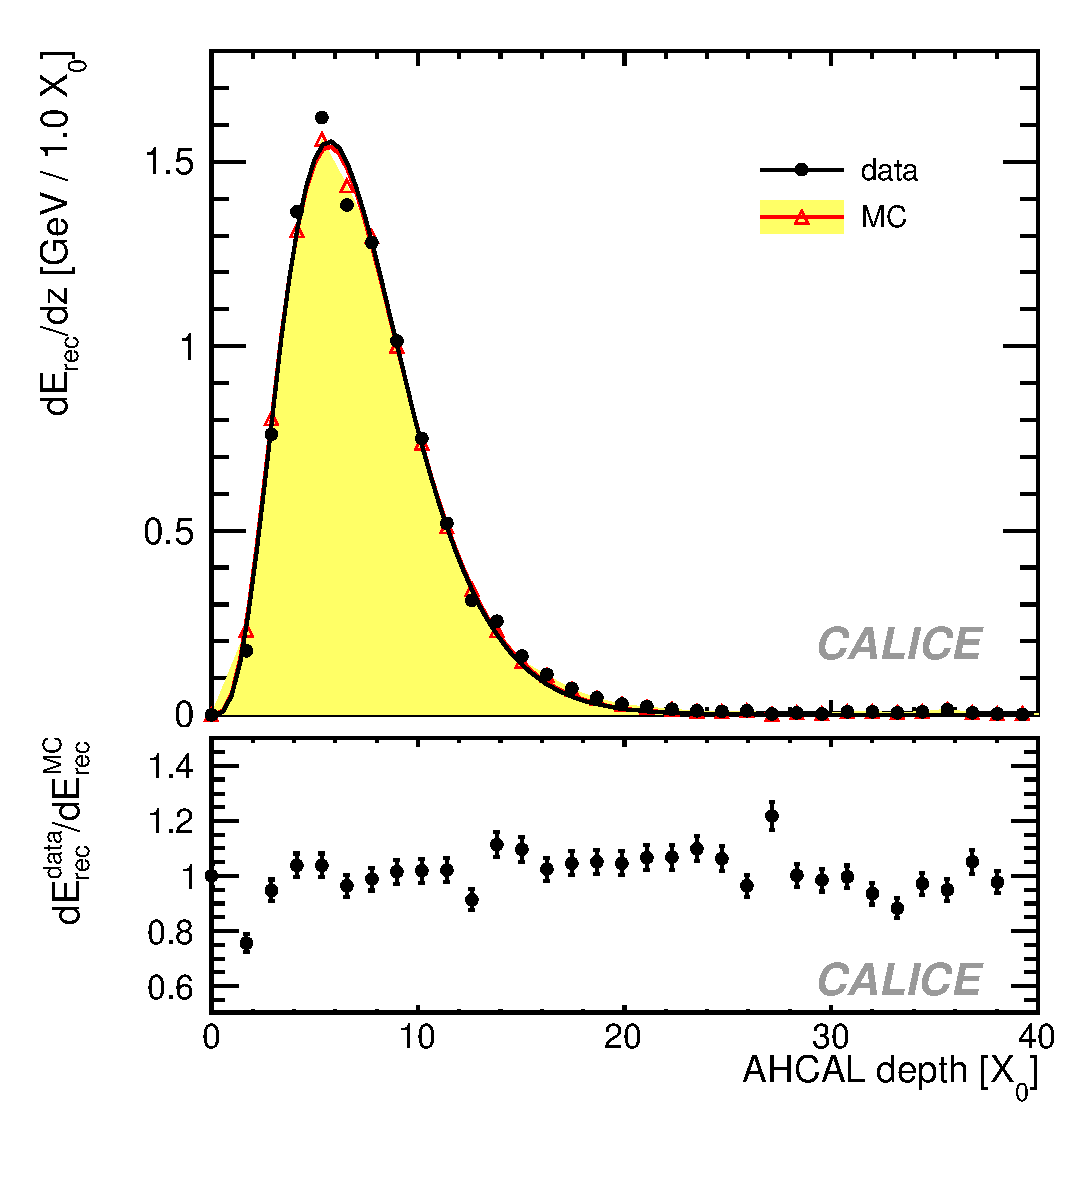
\includegraphics[width=.5\textwidth]{ShowerTh/figs/lProfile.eps}
    \caption{Profile longitudinal des gerbes électromagnétiques induites par des positrons de 10 GeV dans le calorimètre CALICE Fe-AHCAL pour des données expérimentales et une simulation GEANT4.}
    \label{fig:lProfile_e-}
  \end{center}
\end{figure}
La figure~\ref{fig:lProfile_e-} montre un profile longitudinal moyen de cascades électromagnétiques induites par des positrons de 10 $GeV$ dans le calorimètre CALICE Fe-AHCAL \cite{1748-0221-6-04-P04003}. Le profile longitudinal augmente rapidement, présente un maximum (vers $6X_0$ sur la figure~\ref{fig:lProfile_e-}) puis décroit exponentiellement. La première partie correspond à la multiplication des particules secondaires dans la cascade due au rayonnement de freinage des électrons et des positrons et au phénomène de création de paire ($\gamma\rightarrow e^+e^-$). L'énergie par particule secondaire diminue pendant le développement de la cascade. Le maximum est atteint lorsque l'énergie moyenne des particules secondaires est en dessous de l'énergie critique $\epsilon_c$ (voir section~\ref{sec.charged_in_matter}). Après ce maximum, le nombre de particules filles décroit progressivement en utilisant les processus décrits dans les sections~\ref{sec.charged_in_matter} et \ref{sec.photon_in_matter}.

Le développement latérale des gerbes hadroniques a plusieurs causes. À haute énergie, le photon rayonné par un électron (Bremsstrahlung) est émis avec un angle par rapport à la trajectoire de l'électron. Les électrons et les positrons produits lors des processus de création de paire sont émis avec des angles par rapport à la trajectoire du photon. À basse énergie, les électrons et les positrons font des diffusions multiples. De plus, les électrons éjectés des atomes dans les interactions de diffusion Compton et photo-électrique sont émis de façon isotrope. Le développement latérale des gerbes hadroniques est décrit par le profile latéral ou transversale. Cette variable correspond à la quantité d'énergie déposée dans des tranches de l'absorbeur en fonction de la distance à l'axe de la cascade. 
\begin{figure}[!h]
  \begin{center}
    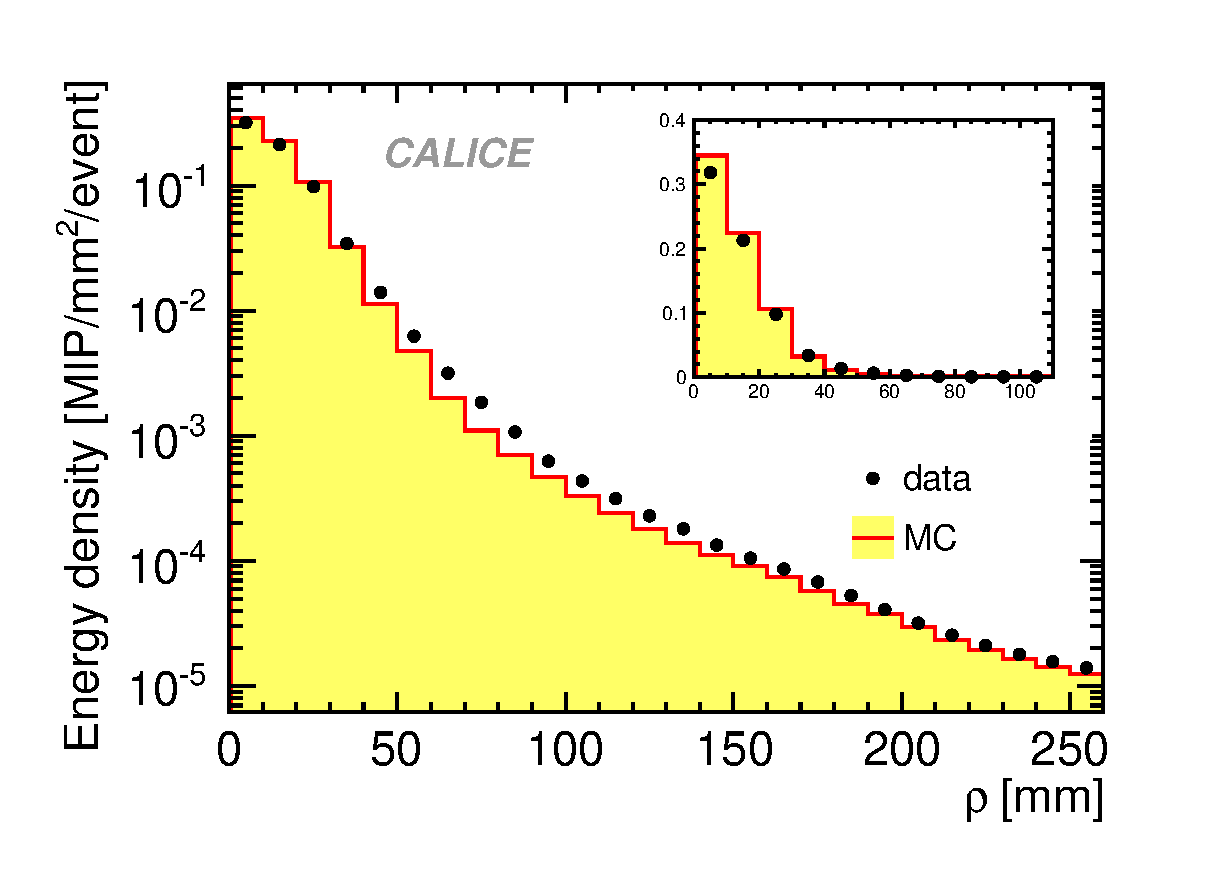
\includegraphics[width=.5\textwidth]{ShowerTh/figs/transverseProfile_15gev_1cm.eps}
    \caption{Profile transversale des gerbes électromagnétiques induites par des positrons de 15 GeV dans le calorimètre CALICE Fe-AHCAL pour des données expérimentales et une simulation GEANT4.}
    \label{fig:tProfile_e-}
  \end{center}
\end{figure}
La figure~\ref{fig:tProfile_e-} présente un profile transversale moyen de cascades électromagnétiques induites par des positrons de 10 $GeV$ dans le calorimètre CALICE Fe-AHCAL \cite{1748-0221-6-04-P04003}. Le profile transversale présente un cœur à faible distance de l'axe de la cascade où un large fraction de l'énergie est déposée. 

\section{Gerbes hadroniques}
\label{sec.hadron_shower}
Le phénomène de gerbe hadronique s'observe dans les expériences de physique des particules où des hadrons de haute énergie sont créés dans des jets. Ces hadrons voyagent jusque dans les calorimètres, interagissent avec l'absorbeur des calorimètres et déclenchent le phénomène de gerbe hadroniques. Le phénomène de cascade hadronique s'observe aussi dans l’atmosphère lorsqu'un rayon cosmique pénètre et interagit dans l'atmosphère. Les rayons cosmiques sont des photons, des protons, des noyaux d'hélium, des électrons... Ils sont principalement générés à l'extérieur du système solaire. La gamme d'énergie des rayons cosmiques varie de quelques $GeV$ à des énergie allant jusqu'à $10^{12}\ GeV$. 
\subsection{Développement d'une cascade hadronique}
Les cascades hadroniques sont plus compliquées que les cascades électromagnétiques. Elles sont initiés par un hadron de haute énergie qui interagit avec un noyau du milieu. Cette interaction crée de nombreuses particules filles. Si l'énergie des particules secondaires est suffisante, de nouvelles réactions avec les noyaux du milieu créent de nouvelles particules. Ce processus continue jusqu'à ce que l'énergie des particules secondaires soit insuffisante pour déclencher les réactions de multiplication. Les processus de basse énergie présentés dans la section~\ref{sec.particle_in_matter} complètent la cascade hadronique. 

Une fraction de l'énergie de la gerbe hadronique est invisible. En effet, nous avons vus que les neutrons et les protons peuvent être capturer par les noyaux du milieu. Les neutrons peuvent aussi interagir et donc être détectés avec du retard et éloignés du reste de la cascade. De plus, les pions chargés qui sont abondamment produits dans la cascade, se désintègrent en muons et neutrinos. Les muons interagissent avec la matière uniquement par ionisation et l'énergie portée par ces muons peut s'échapper du détecteur et détériorer la mesure de l'énergie du hadron incident. Les neutrinos n'interagissent presque pas avec la matière et s'échappe du détecteur. Enfin, pendant le processus de multiplication des particules, des particules se désintégrant électromagnétiquement sont créées. Les produits de désintégration de ces particules constituent la fraction électromagnétique des gerbe hadroniques. La figure~\ref{fig:hadron_shower} montre un schéma d'un développement d'une gerbe hadronique. Les différentes composantes de la cascade sont mis en évidence.
\begin{figure}[!h]
  \begin{center}
    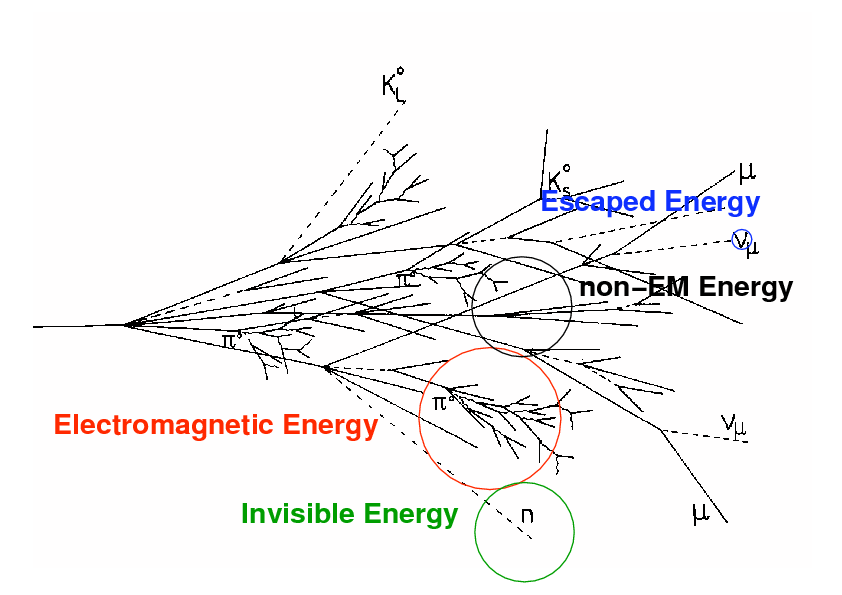
\includegraphics[width=.7\textwidth]{ShowerTh/figs/had-shower.png}
    \caption{Schéma du développement d'une gerbe hadronique.}
    \label{fig:hadron_shower}
  \end{center}
\end{figure}

Les nombreux phénomènes rencontrés dans les gerbes hadroniques introduisent une grande diversité dans le développement d'une cascade. La forme des cascades et la réponse des calorimètres dépend fortement de la proportion des différents processus d'interaction. Tout ceci fait qu'il est très compliqué de mesurer très précisément l'énergie des gerbes hadroniques et de les simuler. 

\subsection{Fraction électromagnétique}
Nous avons déjà mentionné qu'une partie des hadrons créés dans la cascade hadronique se désintègrent électromagnétiquement. C'est particulièrement le cas pour les $\pi_0$s et les $\eta$s. Ces deux particules se désintègrent essentiellement en photons. Ces photons initient ensuite une cascade électromagnétiques si ils ont suffisamment d'énergie. La fraction électromagnétique $f_{em}$ correspond au rapport entre l'énergie déposée électromagnétiquement et l'énergie totale déposée. Malgré les nombreuses fluctuations dues au processus d'hadronisation dans les gerbes hadroniques, un schéma simple permet de donner une approximation de la fraction électromagnétique. Pour chaque collision entre un hadron incident et un noyau du milieu, en moyenne $1/3$ de l'énergie est utilisée pour produire des $\pi_0$s \cite{Gabriel}. Les autres hadrons produits, des pions chargées, vont faire des collisions et $1/3$ de l'énergie sera utiliser pour créer d'autre $\pi_0$. Après $n$ étapes, la fraction électromagnétique vaut en moyenne:
\begin{equation}
  f_{em}=1-(1-\frac{1}{3})^n
\end{equation}
Cette description très simple de la fraction électromagnétique est évidement à corriger. Les hadrons produits ne sont pas que des pions chargées et neutres. Les hadrons chargées déposent de l'énergie par ionisation entre deux collisions. Le nombre moyen de particules secondaires produites par collision varie avec l'énergie du hadron incident. La fraction électromagnétique moyenne augmente donc avec l'énergie. L'équation suivante permet de tenir compte de ces quelques remarques \cite{Gabriel}:
\begin{equation}
  f_{em}=1-(1-\frac{E}{E_0})^{k-1}
\end{equation}
où $E_0$ correspond à l’énergie moyenne nécessaire pour produire un $\pi_0$ et $k$ dépend du nombre moyen de hadrons produits par collision. 

\subsection{Longueur d'interaction}
La longueur d'interaction $\lambda_I$ est la grandeur analogue à la longueur de radiation pour les gerbes hadroniques. Elle est définit comme la longueur moyenne nécessaire qu'un hadron de haute énergie doit parcourir dans un matériau avant de déclencher un réaction nucléaire. La longueur d'interaction est inversement proportionnelle à la section efficace totale de collision $\sigma_{Tot}$ \cite{wigmans}:
\begin{equation}
  \lambda_I=\frac{A}{N_A\sigma_{Tot}} \propto A^\frac{1}{3}
\end{equation}
La section efficace totale varie avec la taille du noyau cible. Elle varie donc comme $r^2$, où $r$ est le rayon du noyau. Le volume du noyau ($\propto r^3$) est proportionnel au nombre de nucléon $A$. La section efficace totale varie aussi avec la taille du hadron incident. La longueur d'interaction est donc légèrement plus grande pour les pions que pour les protons. De même que la longueur de radiation, la longueur d'interaction s'exprime en $g.cm^{-2}$ et il suffit de diviser par la densité pour obtenir une grandeur homogène à une longueur. 
\begin{table}[!ht]
  \begin{center}
    \begin{tabular}{c|c|c|c}
      Matériau & Densité ($g.cm^{-3}$) & $\lambda_I$ ($g.cm^{-2}$) & $\lambda_I$ (cm)\\
      \hline
      Eau & $1.000$ & $115.2$ & $115.2$ \\
      Carbone (graphite) & $2.210$ & $117.8$ & $53.30$ \\
      Aluminum & $2.699$ & $136.7$ & $50.64$ \\
      Fer & $7.874$ & $169.8$ & $20.42$\\
      Cuivre & $8.960$ & $165.9$ & $18.51$\\
      Tungsten & $19.30$ & $218.7$ & $11.33$\\
      Plomb & $11.35$ & $226.2$ & $19.93$\\
      Uranium & $18.95$ & $235.3$ & $12.42$\\
    \end{tabular}
  \end{center}  
  \caption{Longueur d'interaction pour différents matériaux.}
  \label{tab.lI}
\end{table}
Le tableau~\ref{tab.lI} présente les longueurs d'interaction pour les pions pour différents matériaux.

\subsection{Profiles des gerbes hadroniques}
Pour les gerbes hadroniques, les profiles longitudinales et latérales sont définies comme pour les gerbes électromagnétiques. 
\begin{figure}[!h]
  \begin{center}
    \includegraphics[width=.6\textwidth]{ShowerTh/figs/fig_7a_lp.pdf}
    \caption{Profile longitudinal des gerbes hadroniques induites par des pions de 45 GeV dans le calorimètre CALICE Fe-AHCAL. Le profile relatif au premier plan de détecteur est donnée par l'histogramme plein (en bleu). L'histogramme représenté par la ligne noire correspond au profile longitudinal relatif à la première interaction inélastique.}
    \label{fig:lProfile_pi-}
  \end{center}
\end{figure}
La figure~\ref{fig:lProfile_pi-} montre le profile longitudinale moyen de gerbes hadroniques induites par des pions de 45 $GeV$ dans le calorimètre CALICE Fe-AHCAL \cite{ahcal_pi-_profil}. Le profile longitudinale est présenté relatif au premier plan du calorimètre et relatif au plan de la première interaction inélastique: l'énergie déposée par la trace primaire où le hadron incident n'interagit que par ionisation, n'est pas pris en compte. Comme pour les cascades électromagnétiques, le profile longitudinal des gerbes hadroniques augmente jusqu'à un maximum puis décroit exponentiellement. La décroissance est plus progressive que pour les gerbes électromagnétiques. 

\begin{figure}[!h]
  \begin{center}
    \includegraphics[width=.5\textwidth]{ShowerTh/figs/eudet_fig_11_rprof_18_FTF_BIC.pdf}
    \caption{Profile latérale des gerbes hadroniques induites par des pions de 18 GeV dans le calorimètre CALICE Fe-AHCAL pour des données expérimentales et une simulation GEANT4}
    \label{fig:tProfile_pi-}
  \end{center}
\end{figure}
La figure~\ref{fig:tProfile_pi-} présente le profile latérale moyen de gerbe hadroniques de 18 $GeV$ dans le calorimètre CALICE Fe-AHCAL \cite{ahcal_pi-_profil}. Les gerbes hadroniques possèdent aussi un cœur où la densité d'énergie déposée est importante. La fraction électromagnétique est contenue dans de cœur. L'énergie déposée décroit exponentiellement lorsqu'on s'éloigne du cœur de la cascade. Notons que les profils transversaux que nous observerons avec le SDHCAL seront sensiblement différent. Avec le mode de lecture semi-digital, le nombre de coups dans des anneaux concentriques autour de l'axe de la cascade sera compté et définira le profile transversale. Le nombre de coups proche de l'axe des gerbes hadroniques et électromagnétiques sera saturé et la forme des profiles transversaux sera sensiblement différentes.
